\subsection[First Criterium Start]{The First Criterium Start}

\subsubsection{T-15 Minutes}

Assuming no delays%
\sidenote{See \textbf{\nameref{subsec:road_pbp_crit_t-20}}}
the \pbproleref{role:primary_promoter} should get the race ready to start:

\begin{enumerate}
  \item Communicate with the \pbproleref{role:registrar} to close registration%
    % TODO: document when to close registration as a regulation, link
    \sidenote{Registration at ECCC events traditionally closes 15 minutes before the start of the race.}
  \item Announce a first call to staging%
    \sidenote{Try to keep announcements gender-neutral: ``First call for staging for those racing in the Men's C/D field''}
\end{enumerate}

\subsubsection{T-10 Minutes}

The \pbproleref{role:chief_ref} and \pbproleref{role:secondary_promoter} should start getting riders lined up.
Each should be looking to see if any numbers are incorrectly pinned - with ten minutes, issues can be quickly addressed
without delaying the race.

The Announcer should announce a final call to staging.

\subsubsection{T-5 Minutes}

Once the majority of participants have lined up, the \pbproleref{role:primary_promoter} should record the bib numbers
of each rider on the start line.
The \pbproleref{role:primary_promoter} can record the numbers via a voice recording, typing them in to a spreadsheet,
or by using a custom app%
\sidenote{Flyyn/The Results Van are working on an app for this.}.

If any riders need to be talked to%
\sidenote{There are various reasons why riders may need to be found before starting: missing waivers or payment, unaddressed rule violations in prior races, etc.}
the \pbproleref{role:primary_promoter} should be looking for those numbers as they check the riders.

\index{officiating!refereeing}
The \pbproleref{role:chief_ref} typically gives a series of announcements and rule reminders.
The \pbproleref{role:primary_promoter} should supplement the announcements with any specifics about the course or collegiate cycling points and procedures.

\begin{marginfigure}
  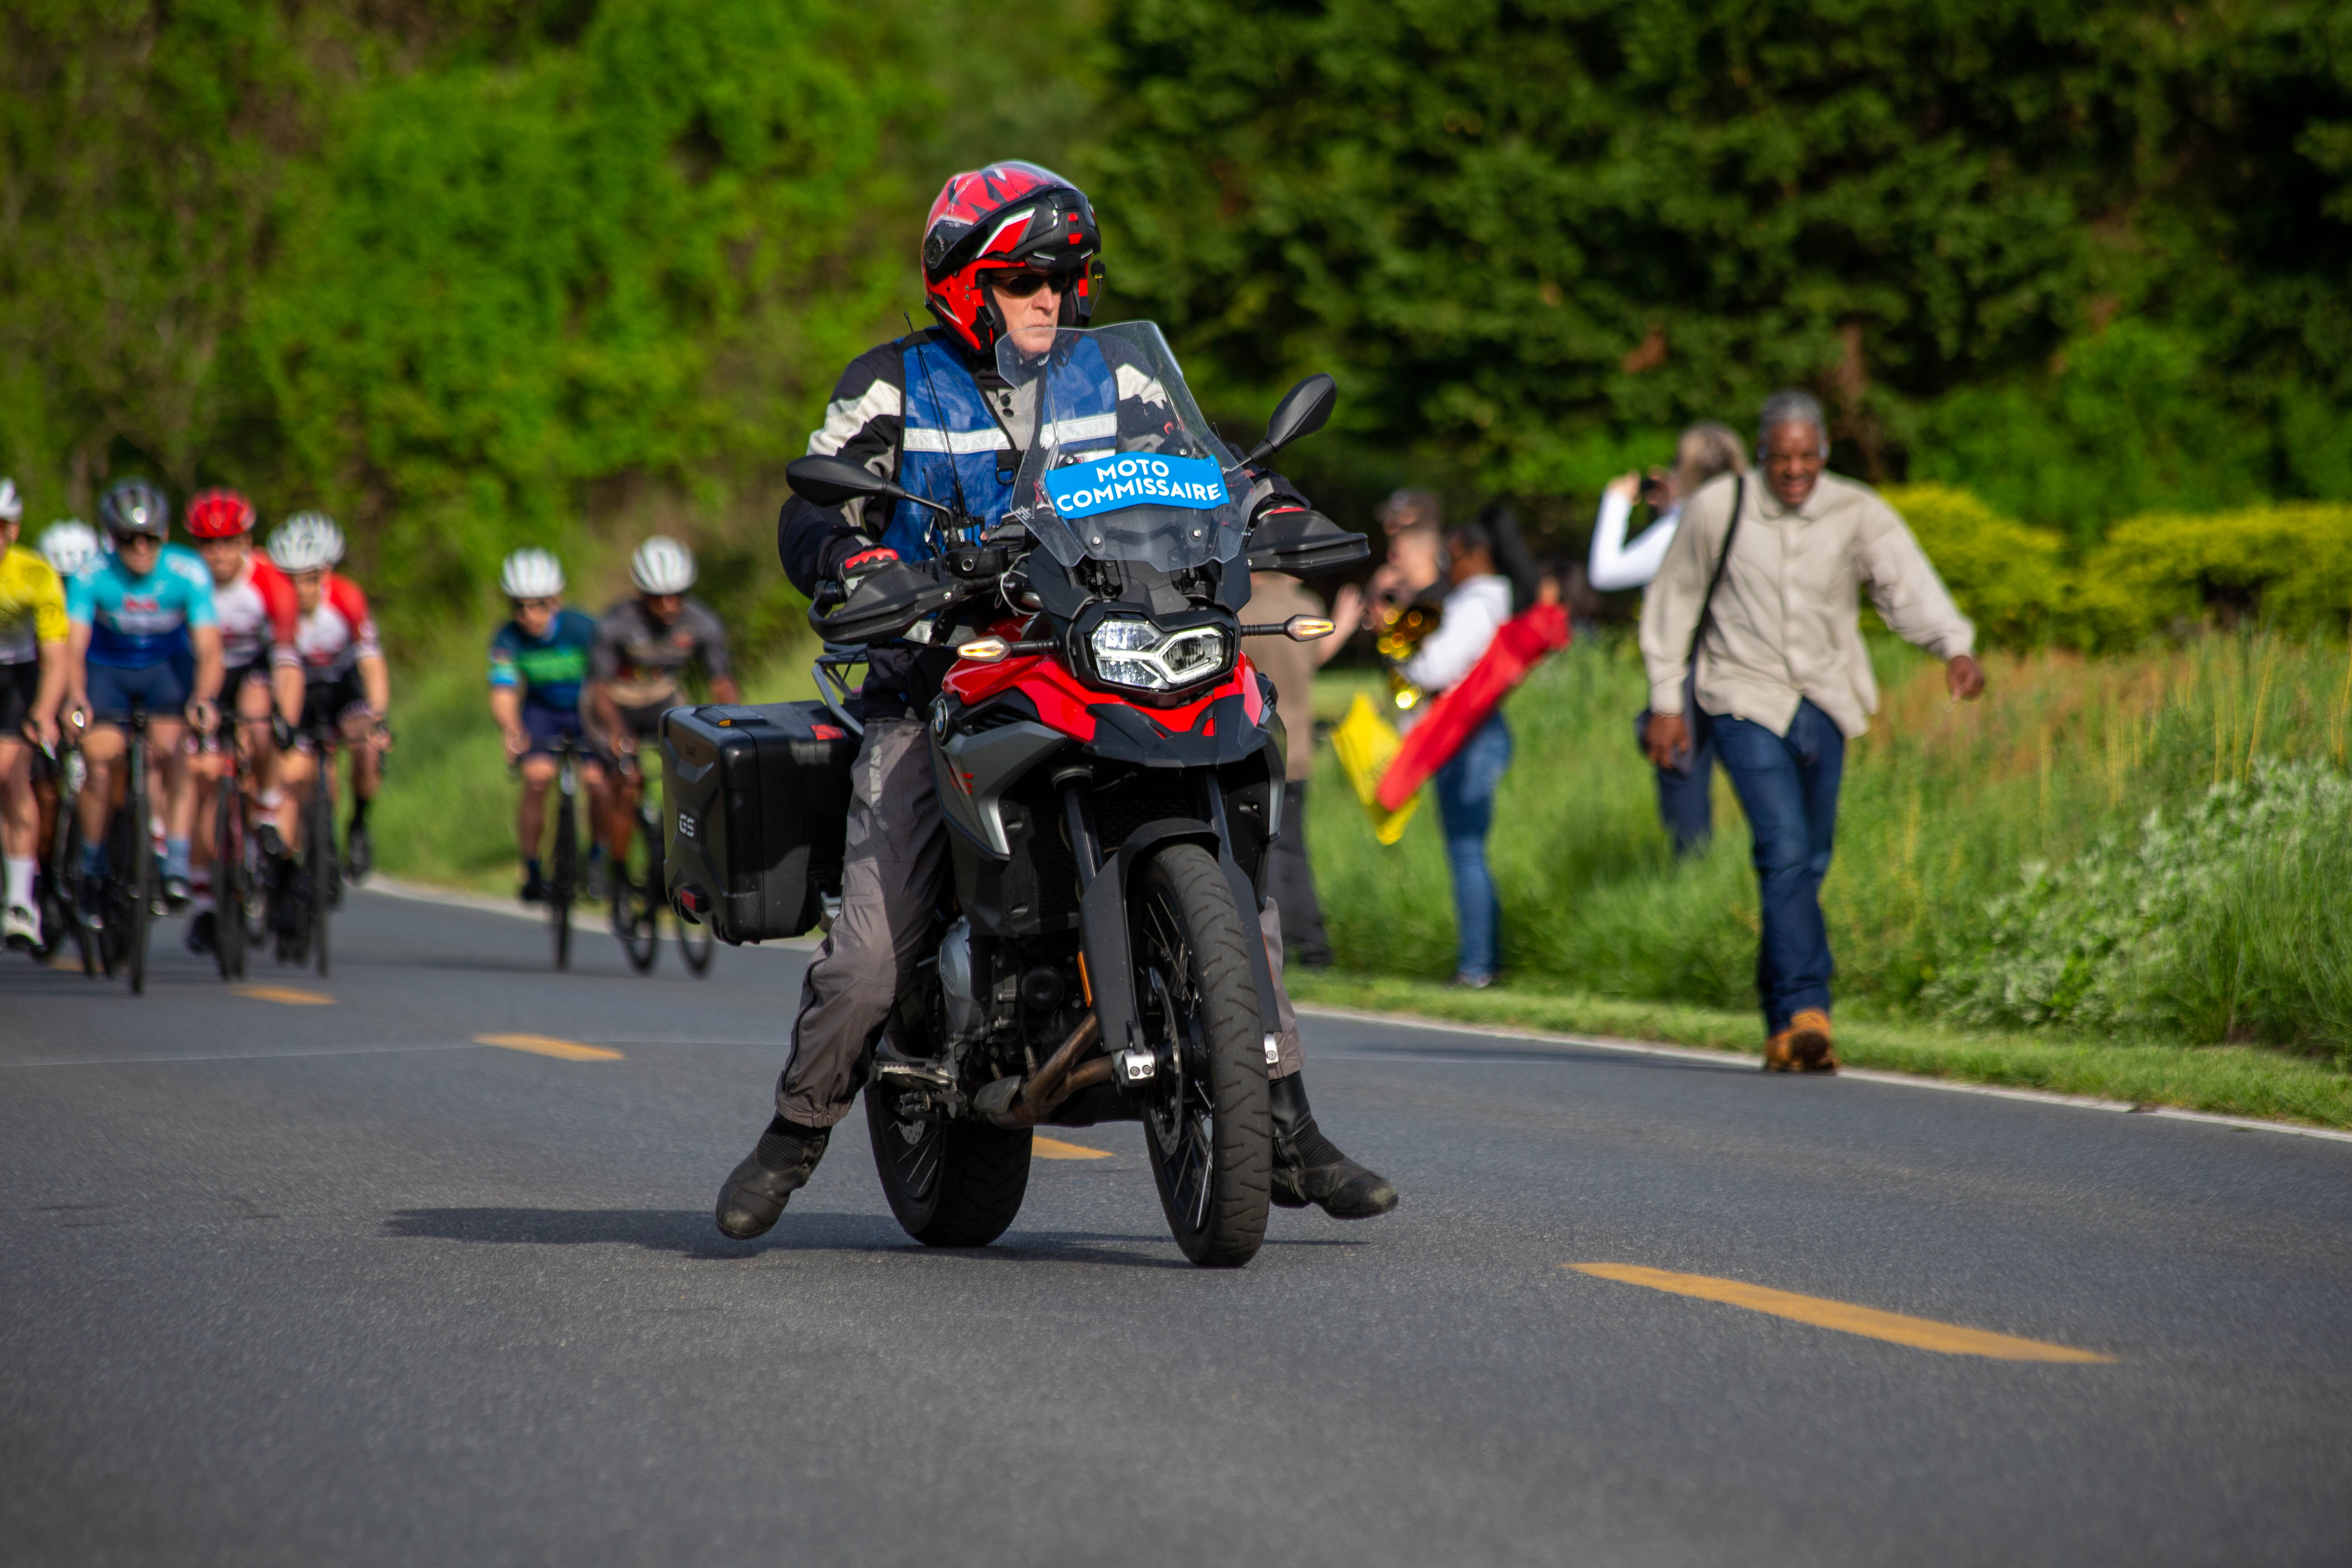
\includegraphics{2023_navy_race_moto_start.jpg}
  \caption[Motorcycle referee starting a race]{From the 2023 Navy Race.\\
            Credit: Chris Azzam}
  \labfig{pbp_road_moto_start}
\end{marginfigure}

\index{officiating!refereeing}
Once all announcements are given, the \pbproleref{role:chief_ref} should announce how much longer it will be until the start whistle,
and the riders will be waiting for the whistle (\reffig{pbp_road_moto_start}).

\subsubsection{T-0 Minutes}

\index{officiating!refereeing}
The \pbproleref{role:chief_ref} will blow the whistle (ideally on a open microphone, so everyone with a radio can hear),
and the race will start!

The \pbproleref{role:secondary_promoter} and \pbproleref{role:assistant_promoter} should watch the first 30-45 seconds of the race
to ensure that all participants have a smooth and safe start.

\subsubsection{T+5 Minutes}

Soon after the race starts, the \pbproleref{role:primary_promoter} should ask the \pbproleref{role:registrar} for a final list of
participants in the race, and get the information to the Timing Company so they have a complete start list.
